\clearpage
\phantomsection

\addcontentsline{toc}{chapter}{{PHỤ LỤC}}
\chapter*{Phụ lục}
\renewcommand{\thefigure}{A.\arabic{figure}} 
\setcounter{figure}{0}
\begin{enumerate}[A$).$]
	\item {Flow-graph mô phỏng DOA với dữ liệu Matlab trên GNU Radio.
			\par
			\begin{figure} [!h]
			\centering
			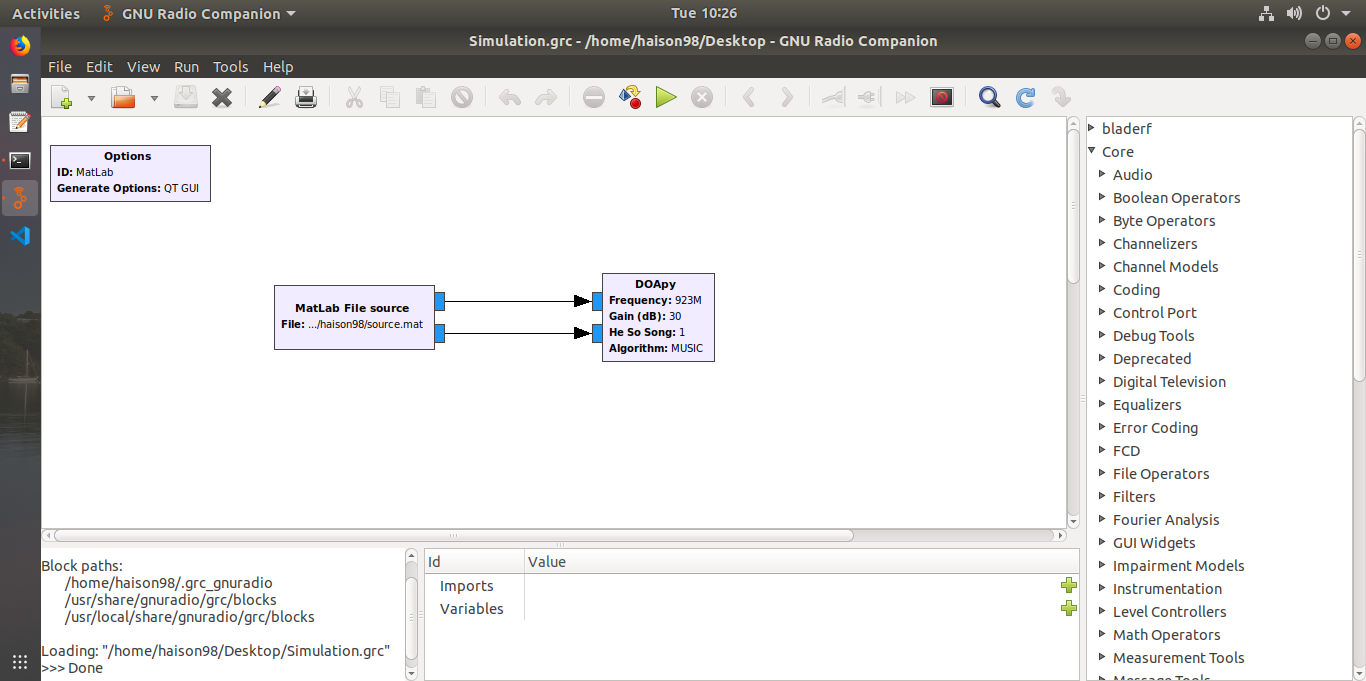
\includegraphics[width=1\linewidth]{figures/simulation1.png}
			\caption{Flow-graph ước lượng DOA với dữ liệu mô phỏng Matlab trên GNU Radio}
			\label{fig:simulation1}
			\end{figure} 
			\newpage}
	\item {
		Mô phỏng dữ liệu thu từ BladeRF, vừa chịu ảnh hưởng từ kênh truyền, vừa chịu ảnh hưởng do sai số phần cứng BladeRF gây ra.
		\renewcommand{\thefigure}{B.\arabic{figure}} 
		\setcounter{figure}{0}
		 \begin{figure}[!ht]
			%\hfill
			\centering
			\subfigure[Mô phỏng tạp âm và nhiễu đa đường]{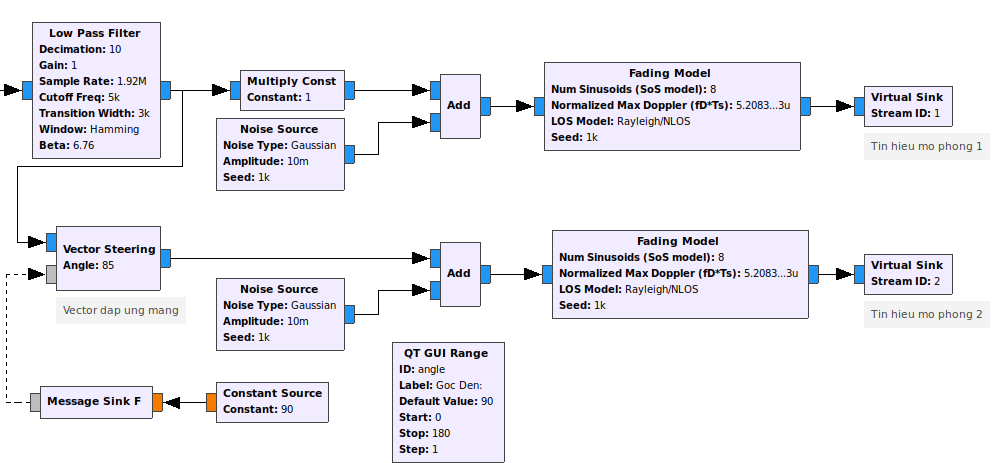
\includegraphics[width=1\linewidth]{figures/channel.png}
				\label{fig:channel}}
			\hfill
			\subfigure[Mô phỏng $\textrm{sample}_\textrm{offset}$ và $\textrm{phase}_\textrm{offset}$]{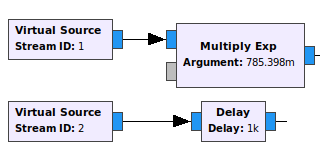
\includegraphics[width=0.5\linewidth]{figures/sampleandphase.png}\label{fig:sampleandphase}}
			\hfill
			\caption{Mô phỏng dữ liệu BladeRF qua kênh truyền}
			\label{fig:bladesimu}
		\end{figure}
	\newpage
	}

	\item {
		Flow-graph điều chế tín hiệu NBFM:
		\renewcommand{\thefigure}{C.\arabic{figure}} 
		\setcounter{figure}{0}
\begin{figure} [!h]
	\centering
	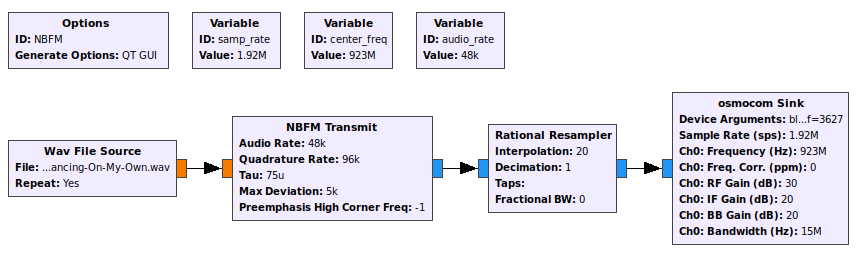
\includegraphics[width=1\linewidth]{figures/NBFM.png}
	\caption{Flow-graph truyền tín hiệu NBFM}
	\label{fig:NBFM}
\end{figure}
	\newpage	
}
	
	\item {
		Flow-graph của hệ DOA trên BladeRF, các khối tương ứng với chức năng chính:
		%\renewcommand{\labelitemi}{$-$}
		\begin{itemize}
			\item Osmosdr Source: khối nguồn lấy dữ liệu trực tiếp từ các SDR, được phát triển dưới dạng mã nguồn mở,  hỗ trợ rất nhiều loại SDR: RTL-SDR, USRP, BladeRF, HackRF, LimeSDR, ... Có sẵn hầu hết các thông số đầu vào như tần số thu, tốc độ lấy mẫu, băng thông, khuếch đại,... tất cả đều trực quan và dễ dàng chỉnh sửa. %APIs
			\item DC Blocker: loại bỏ thành phần một chiều trong tín hiệu.
			\item Low Pass Filter: bộ lọc thông thấp, dễ dàng chuyển đổi $f_\textrm{cut}$ tương ứng với trạng thái đồng bộ hoặc ước lượng DOA của hệ thống.
			\item Virtual Sink/Source: các khối chuyển tiếp dữ liệu, giúp thu gọn và chia luồng dữ liệu để tiện xử lý.
			\item $\textrm{Sample}_\textrm{offset}$: ước lượng mẫu offset do trễ đầu vào.
			\item PCA Phase Diff: tính toán độ lệch pha giữa 2 tín hiệu cho bước đồng bộ SDR.
			\item Probe Signal/Funcion Probe: lưu giá trị đầu vào dưới dạng biến làm thông số cho các khối khác.
			\item DOA/DOA Python: khối ước lượng DOA được viết trên ngôn ngữ tương ứng C++/Python.
			\item QT GUI: các khối hiển thị giao diện người dùng.
		\end{itemize}
		
		
		\renewcommand{\thefigure}{D.\arabic{figure}} 
		\setcounter{figure}{0}
		\afterpage{\clearpage}
		\begin{figure} [!ht]
			\centering
			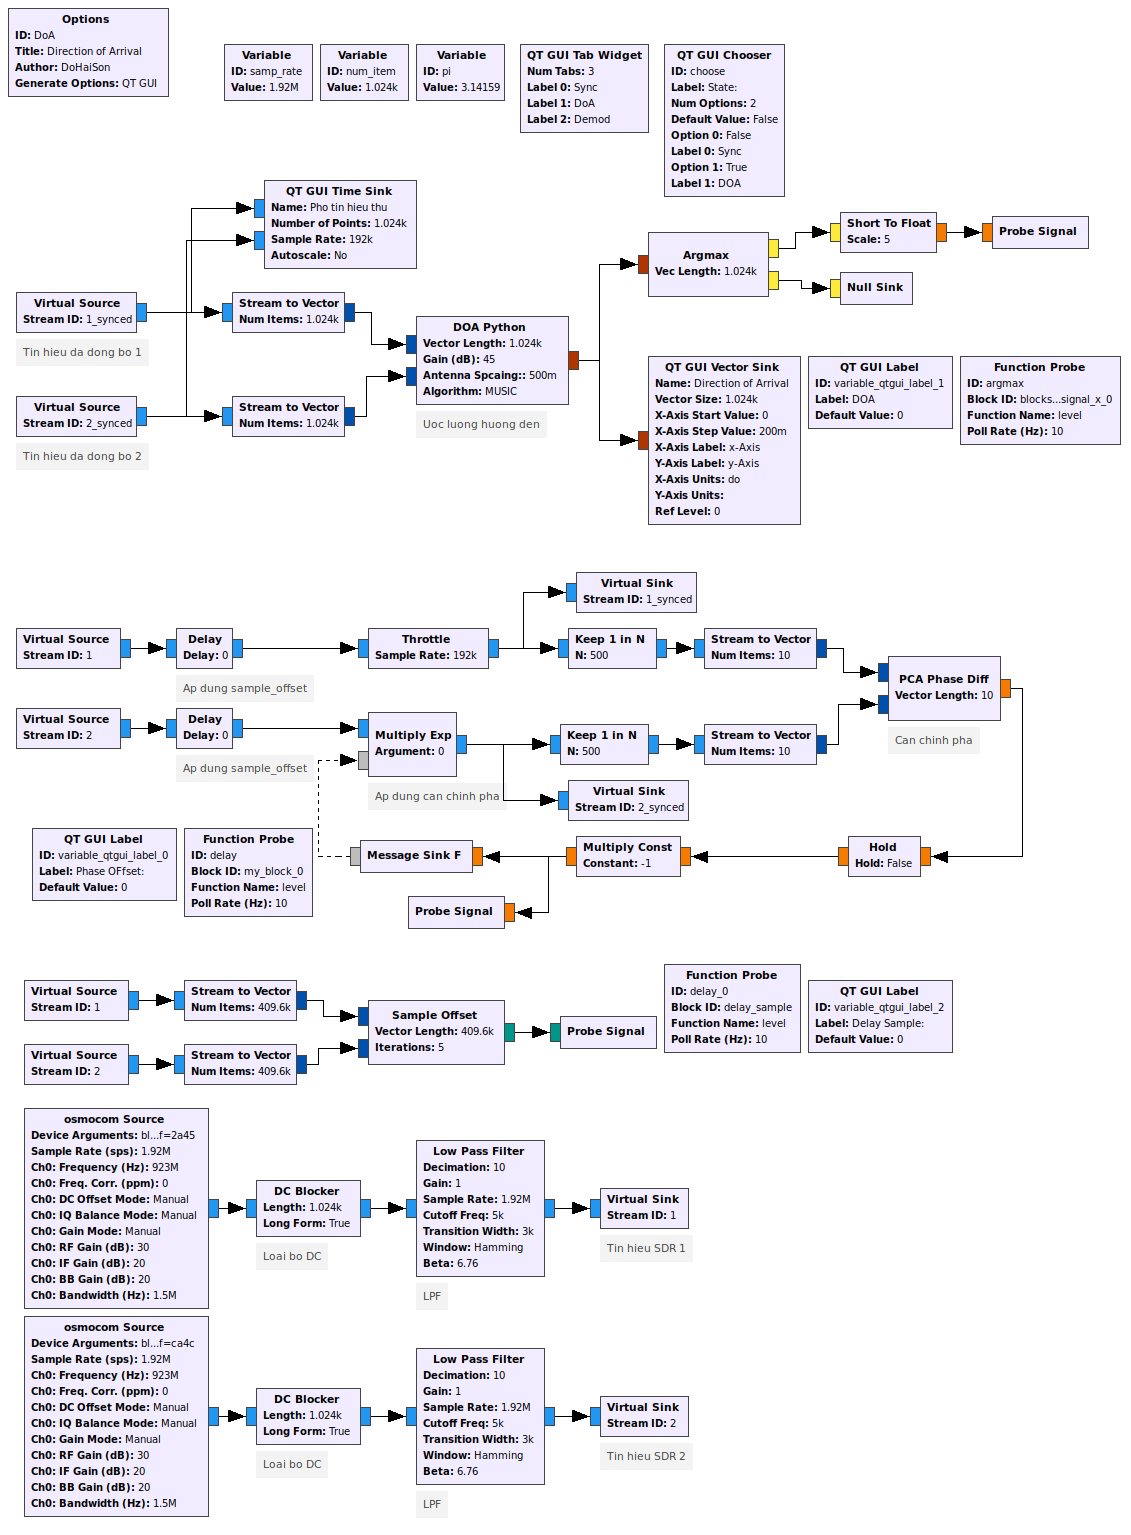
\includegraphics[width=\textwidth,height=\textheight,keepaspectratio]{figures/DoA_FM_grc.png}
			\caption{Flow-graph ước lượng DOA}
			\label{fig:DoA_FM}
		\end{figure}
	\newpage
	}
	
	\item {
		Flow-graph điều chế tín hiệu truyền hình chuẩn DVB-T trên GNU Radio.
	\renewcommand{\thefigure}{E.\arabic{figure}} 
	\setcounter{figure}{0}
	\begin{figure} [!h]
		\centering
		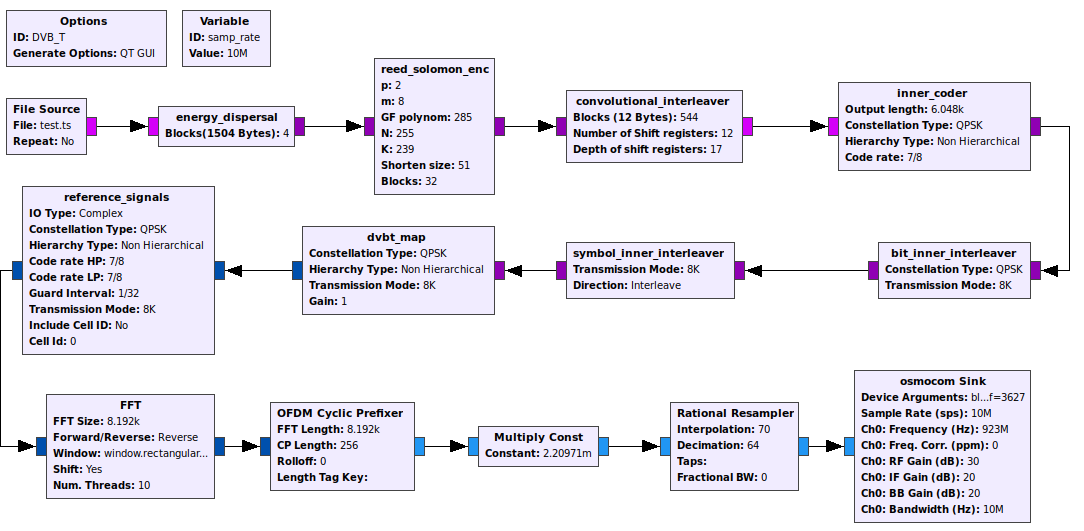
\includegraphics[width=0.95\linewidth]{figures/dvbt.png}
		\caption{Flow-graph truyền tín hiệu DVB-T}
		\label{fig:dvbt}
	\end{figure}	
}
\end{enumerate}